\chapter{Progettazione Logica}
In questo capitolo verrà trattato il passaggio dalla progettazione concettuale alla progettazione logica. Nello schema che seguirà le chiavi primarie saranno identificate con una \underline{sottolineatura} e le chiavi esterne con un *.

\section{Schema Logico}

\begingroup
    \setlength{\tabcolsep}{20pt}
    \renewcommand{\arraystretch}{2.0}
    \begin{xltabular}{\textwidth}{l X}

        \textbf{Contratto} & (\underline{IDContratto}, Tipo, DataFirma, ScadenzaContratto, Stipendio, CF*)
        \newline CF $\rightarrow$ Dipendente.CF \\

        \textbf{Dipendente} & (Nome, Cognome, \underline{CF}, Specializzazione, Ruolo, Ufficio, Mansione) \\
       
        \textbf{Laboratorio} & (\underline{Topic},\underline{Edificio}, \underline{Stanza}) \\
       
        \textbf{Progetto} & (\underline{CUP}, Nome, Budget) 
        \\
        \textbf{Utilizzo} & (CUP*,Topic*,Edificio*,Stanza*)
        \newline CUP$\rightarrow$Progetto.CUP
        \newline (Topic,Edificio,Stanza)$\rightarrow$Laboratorio.(Topic,Edificio,Stanza) \\
        \textbf{Carriera} & (\underline{IDCarriera}, PrimaAssunzione, DataPromozione, RuoloPrecedente, AumentoStipendio, StipendioCorrente, StipendioPrecedente) \\

        \textbf{Possessione} & (IDCarriera*, CF*) 
        \newline IDCarriera$\rightarrow$Carriera.IDCarriera
        \newline CF $\rightarrow$ Dipendente.CF \\ 

        \textbf{Azienda} & (\underline{Nome}, Titolare,\underline{Via}, Civico, CAP, Fatturato) \\

        \textbf{Assunzione} & (Nome*, Via*, CF*) 
        \newline Nome $\rightarrow$ Azienda.Nome
        \newline Via $\rightarrow$ Azienda.Via 
        \newline CF $\rightarrow$ Dipendente.CF \\

        \textbf{Finanziamento} & (Nome*, Via*,CUP*) 
        \newline Nome $\rightarrow$ Azienda.Nome 
        \newline Via $\rightarrow$ Azienda.Via 
        \newline CUP $\rightarrow$ Progetto.CUP \\

        \textbf{Afferenza} & (CF*, Topic*, Edificio*, Stanza*) 
        \newline CF $\rightarrow$ Dipendente.CF 
        \newline (Topic,Edificio,Stanza) $\rightarrow$ Laboratorio.(Topic,Edificio,Stanza)\\
        
        \textbf{Responsabilità} & (CF*, CUP*)
        \newline CF $\rightarrow$ Dipendente.CF 
        \newline CUP $\rightarrow$ Progetto.CUP \\
        
        \textbf{Gestione} & (CF*, Topic*, Edificio*, Stanza*) 
        \newline CF $\rightarrow$ Dipendente.CF 
        \newline (Topic,Edificio,Stanza) $\rightarrow$ Laboratorio.(Topic,Edificio,Stanza) \\
        
        \textbf{Referenza} & (CF*, CUP*)
        \newline CF $\rightarrow$ Dipendente.CF 
        \newline CUP $\rightarrow$ Progetto.CUP \\

    \end{xltabular}
\endgroup

\section{Trigger e Procedure}
\subsection{Indeterminato senza scadenza}
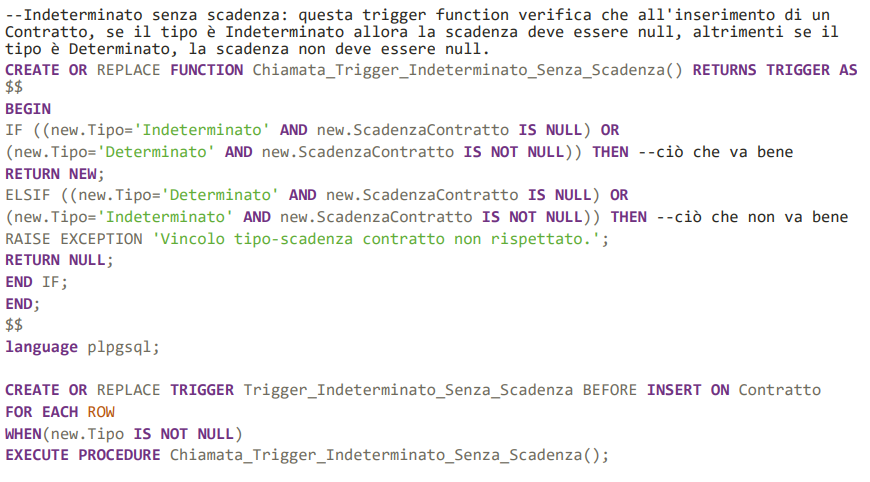
\includegraphics[width=1.2\textwidth]{Immagini/vincolo1.sql}
Esempio di cosa accade se si prova ad inserire un contratto non valido:
\newline\newline
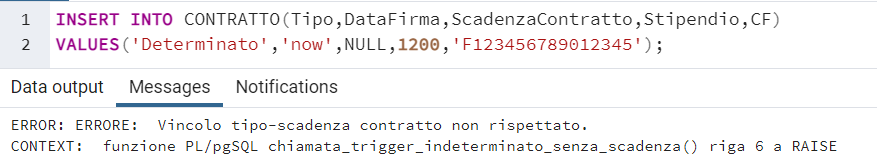
\includegraphics[width=1.2\textwidth]{Immagini/vincolo1}

\subsection{Passaggio a indeterminato}
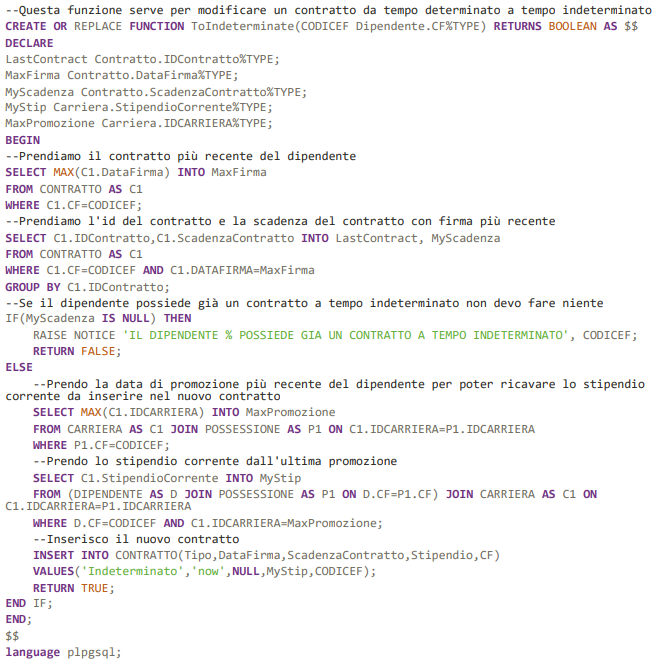
\includegraphics[width=1.2\textwidth]{Immagini/function1.sql}
\newpage
Esempio di cosa accade se si prova a modificare un contratto da determinato a indeterminato:
\newline\newline
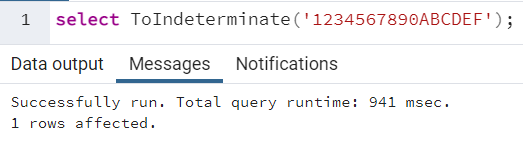
\includegraphics[width=0.8\textwidth]{Immagini/funzione1ok}
\newline\newline
Esempio di cosa accade se si prova a modificare un contratto a indeterminato se è già indeterminato.
\newline\newline
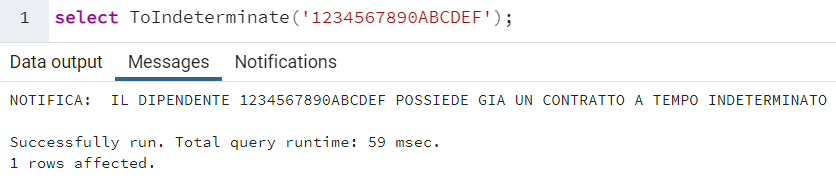
\includegraphics[width=1.1\textwidth]{Immagini/funzione1no}
\subsection{Rinnovo contratto scaduto}
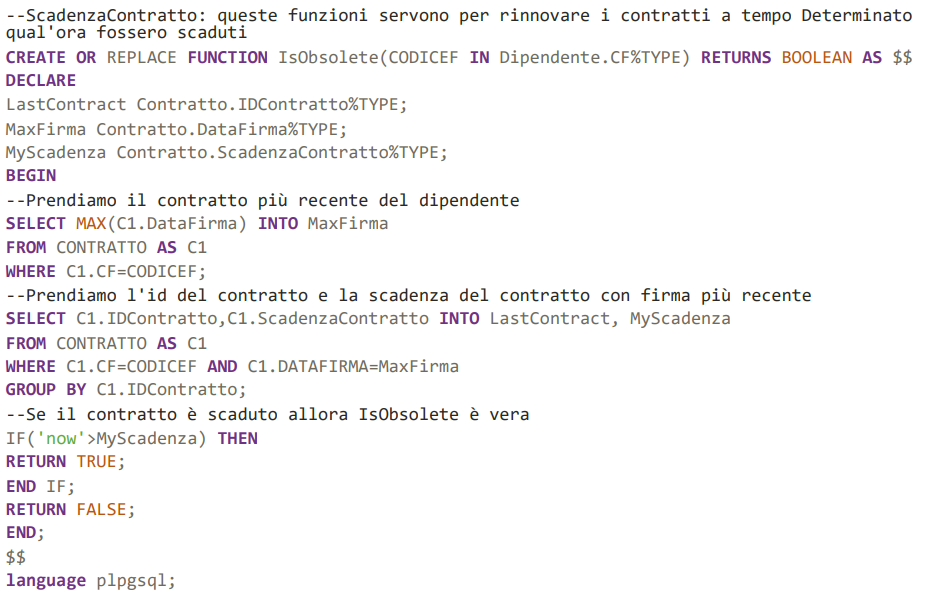
\includegraphics[width=1\textwidth]{Immagini/funzione2.sql}
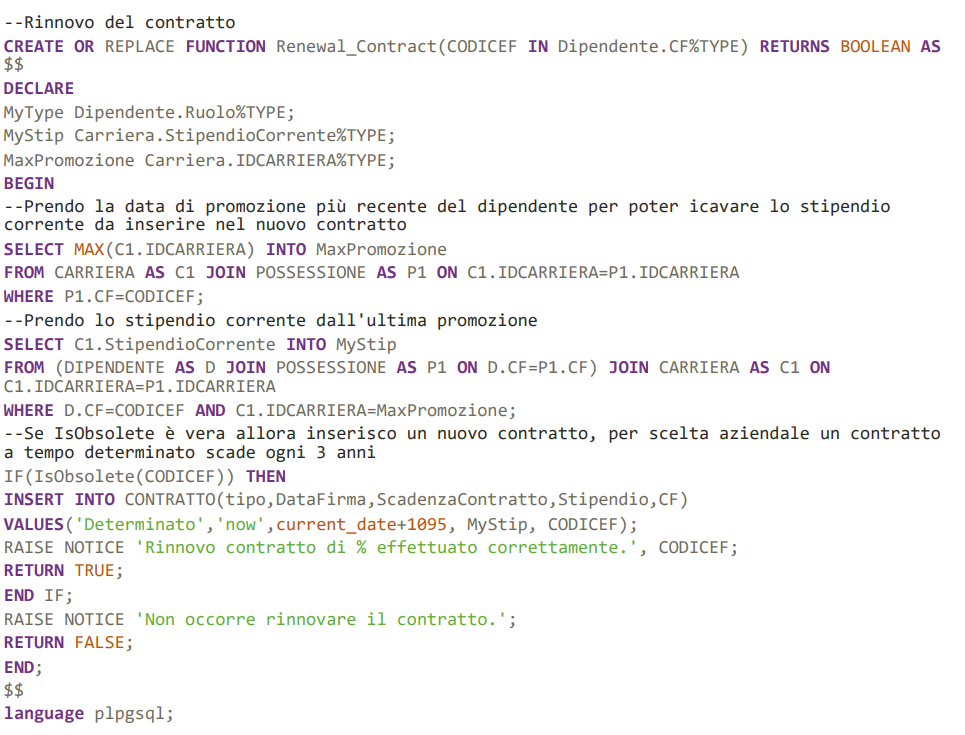
\includegraphics[width=1.1\textwidth]{Immagini/funzione2.1.sql}
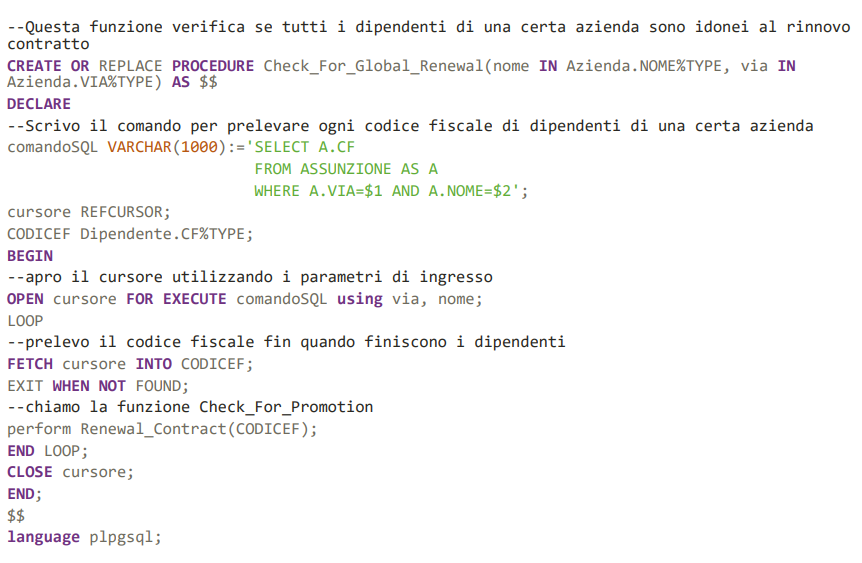
\includegraphics[width=1.1\textwidth]{Immagini/funzione2.2.sql}
\newline\newline
Esempio di cosa accade se rinnovo tutti i contratti scaduti di una certa azienda:
\newline\newline
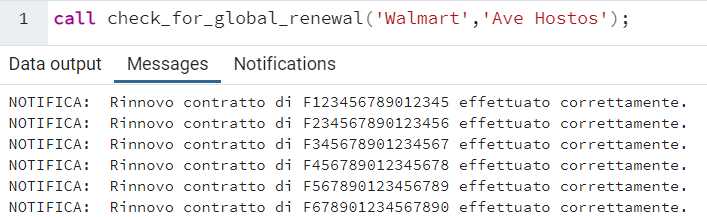
\includegraphics[width=1.1\textwidth]{Immagini/funzione2ok.png}
\subsection{Assunzione dei dipendenti e firma del contratto}
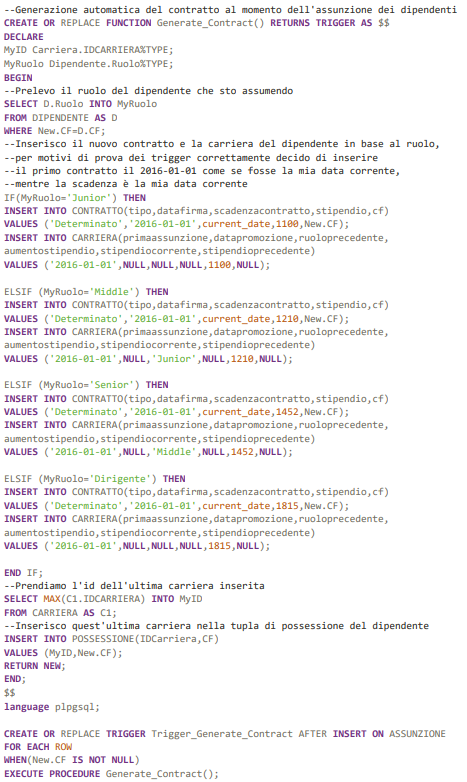
\includegraphics[width=0.9\textwidth]{Immagini/trigger1.sql}
\subsection{Utilizzo laboratori}
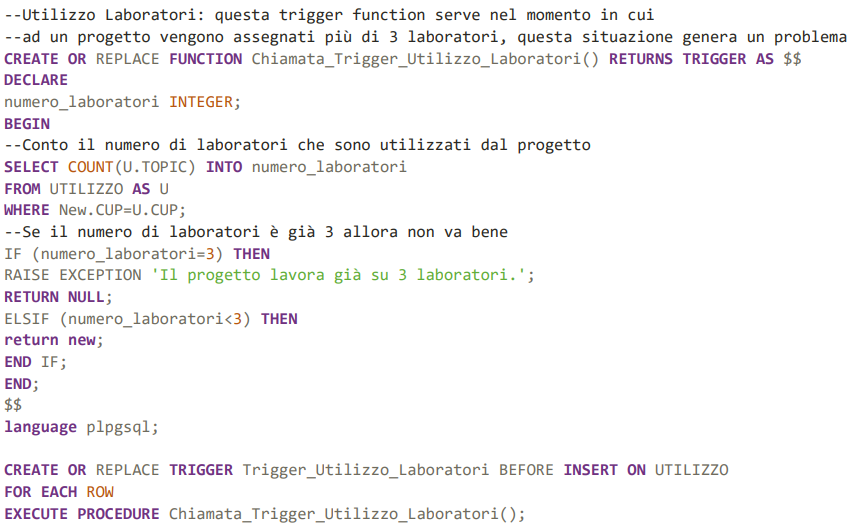
\includegraphics[width=1.1\textwidth]{Immagini/vincolo2.sql}
\newline\newline
Esempio di cosa accade se un progetto tenta di utilizzare più di 3 laboratori:
\newline\newline
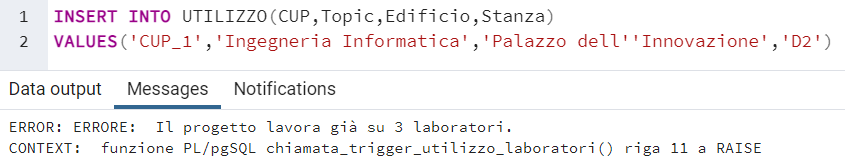
\includegraphics[width=1.1\textwidth]{Immagini/vincolo2}
\subsection{Passaggio a nuovo ruolo}
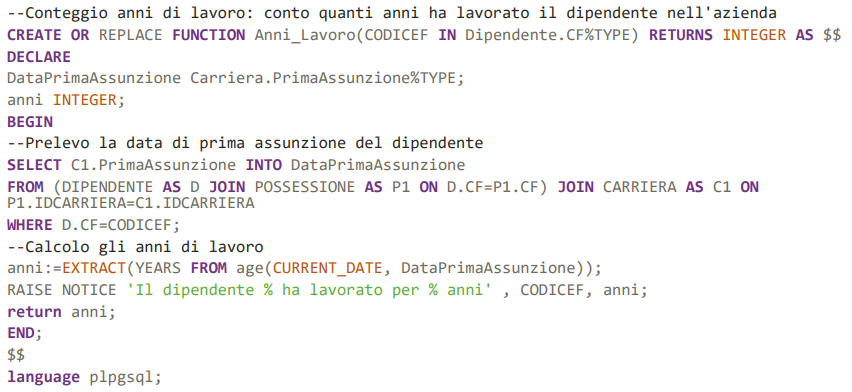
\includegraphics[width=1.1\textwidth]{Immagini/funzione3anni.sql}
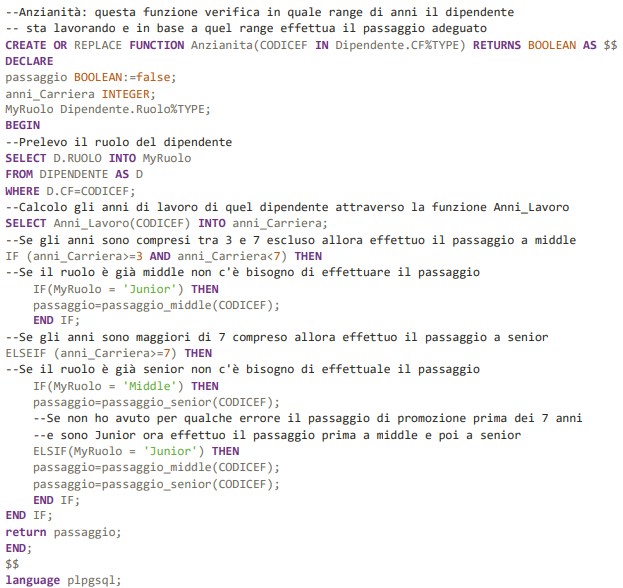
\includegraphics[width=1\textwidth]{Immagini/anzianita.sql}
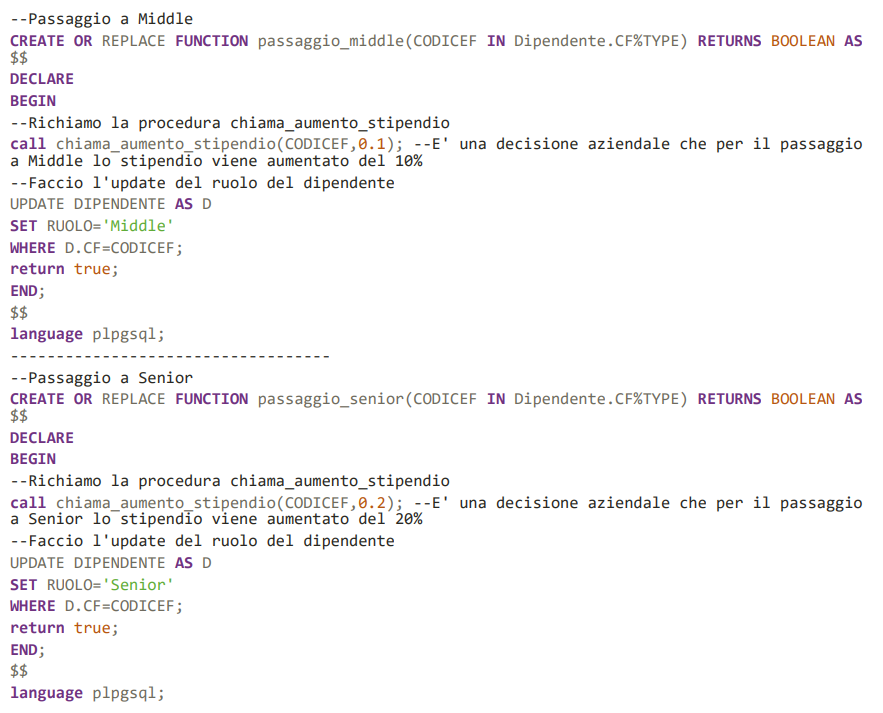
\includegraphics[width=1\textwidth]{Immagini/passaggio.sql}
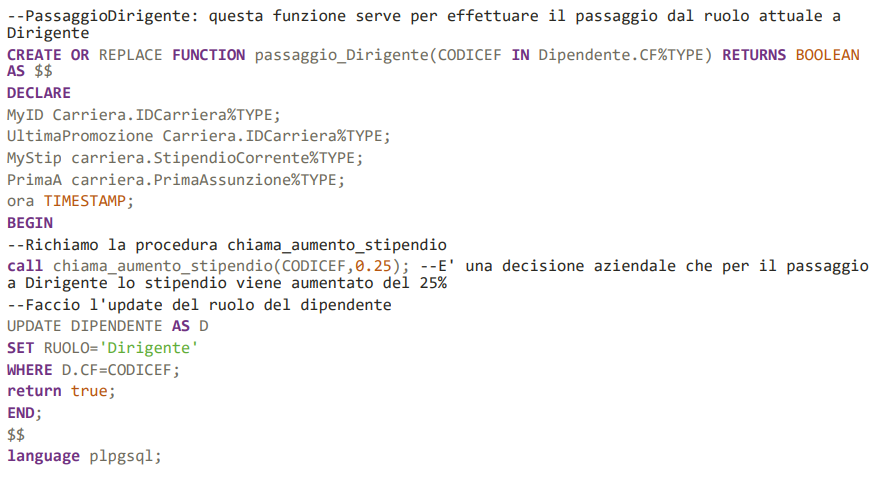
\includegraphics[width=1\textwidth]{Immagini/passaggioDir.sql}
\newpage
Esempio di cosa accade se effettuo un passaggio a Dirigente di un dipendente:
\newline\newline
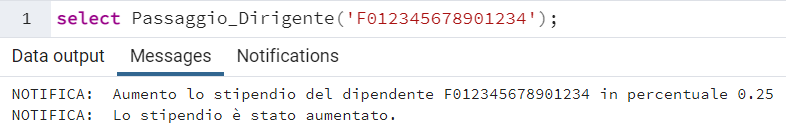
\includegraphics[width=1\textwidth]{Immagini/passaggioDir}

\includegraphics[width=1.2\textwidth]{Immagini/viola}
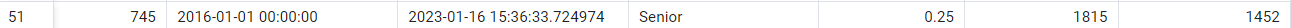
\includegraphics[width=1.2\textwidth]{Immagini/carriera}
\newline\newline
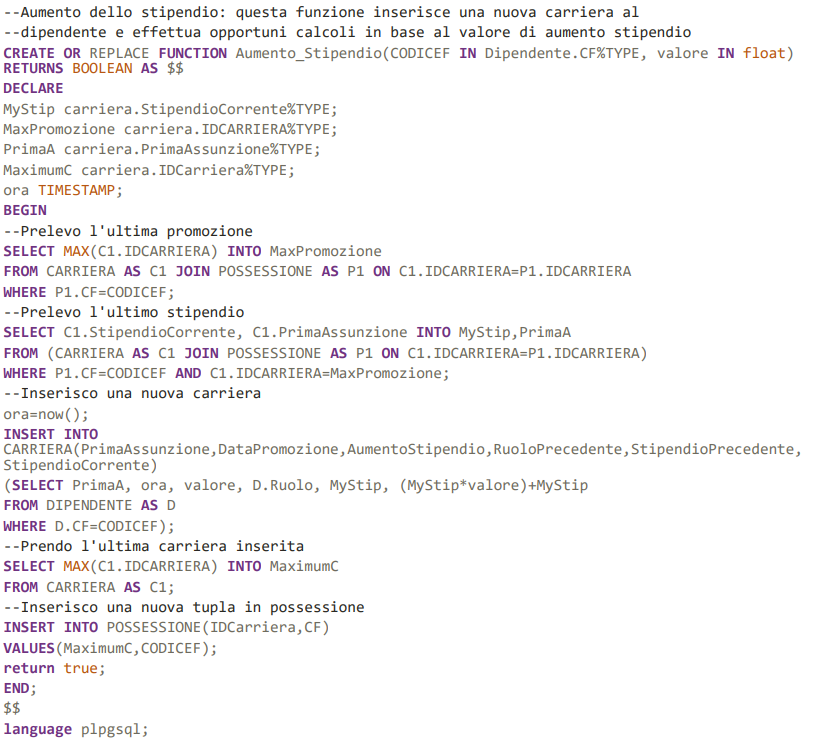
\includegraphics[width=1\textwidth]{Immagini/aumento_stip.sql}
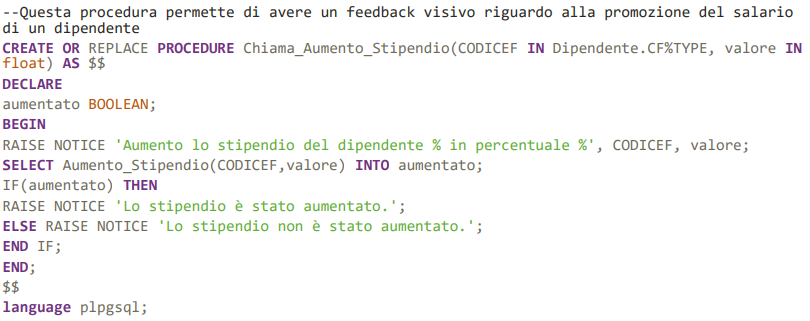
\includegraphics[width=1\textwidth]{Immagini/chiama_aum.sql.png}
Esempio di cosa accade quando aumento lo stipendio di un dipendente:
\newline\newline
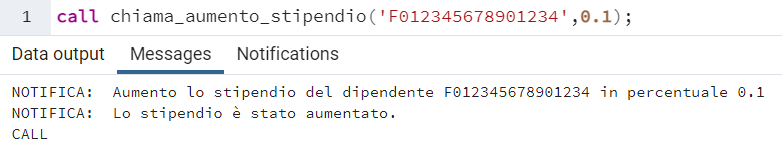
\includegraphics[width=1\textwidth]{Immagini/aum_es.png}

\includegraphics[width=1\textwidth]{Immagini/aum_es2.png}
\newline\newline
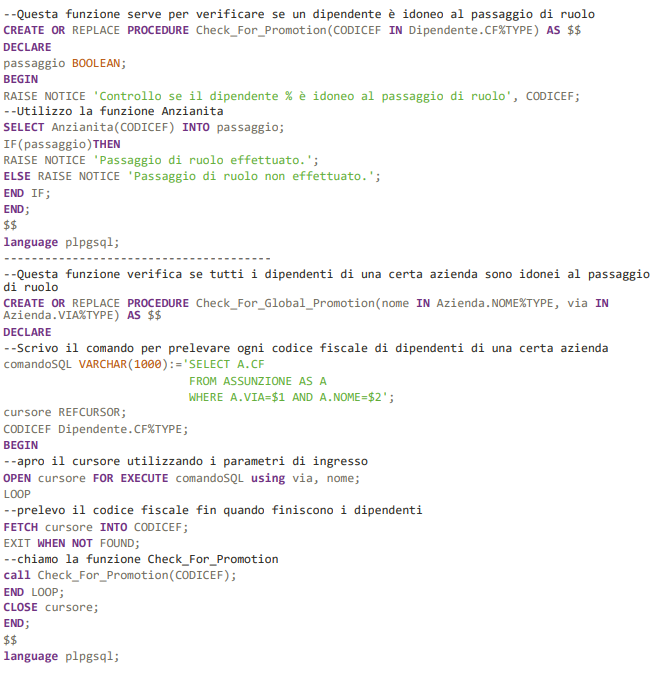
\includegraphics[width=1.2\textwidth]{Immagini/idoneopass.sql}
\newpage
Esempio di cosa accade quando verifico se i dipendenti di un'azienda
sono idonei o meno alla promozione (passaggio di ruolo):
\newline\newline
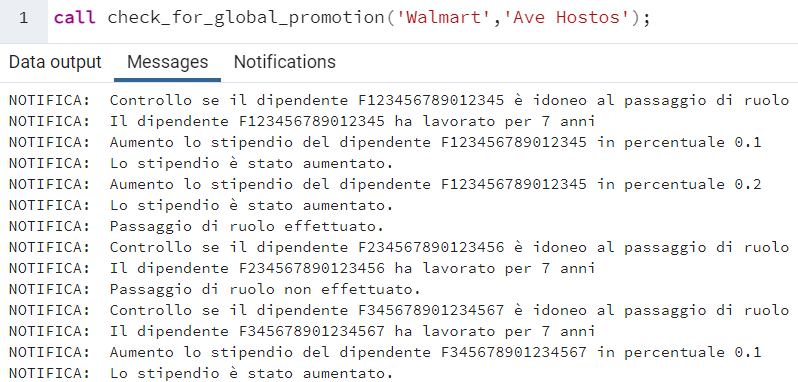
\includegraphics[width=1\textwidth]{Immagini/idonei.png}
\subsection{Consistenza data di prima assunzione}
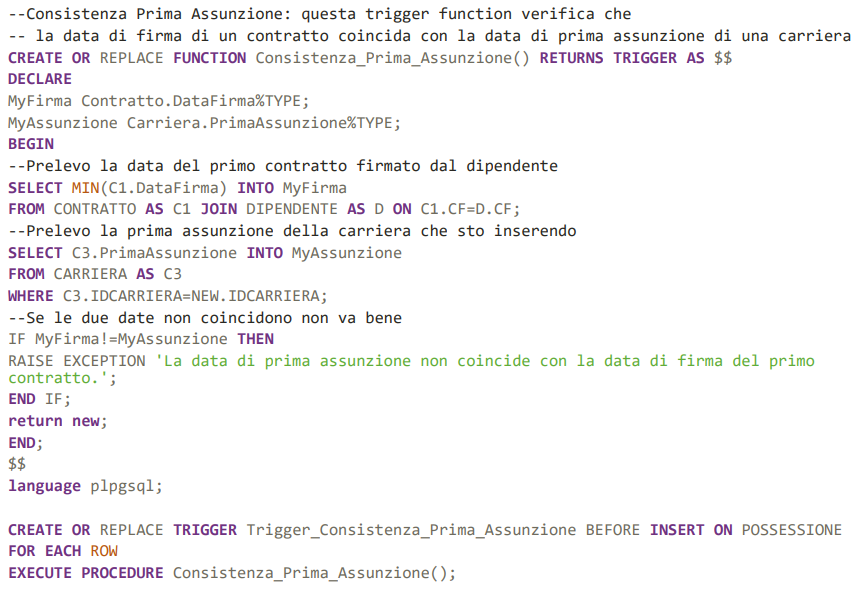
\includegraphics[width=1\textwidth]{Immagini/consistenzadate.sql}
\newpage
Esempio di cosa accade quando provo a collegare una carriera con data di prima assunzione
diversa dalla data di firma del primo contratto di un dipendente:
\newline\newline
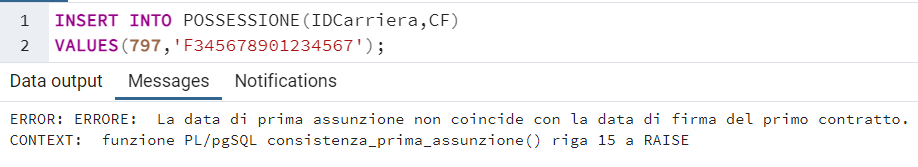
\includegraphics[width=1\textwidth]{Immagini/consdatees}
\subsection{Responsabilità progetti}
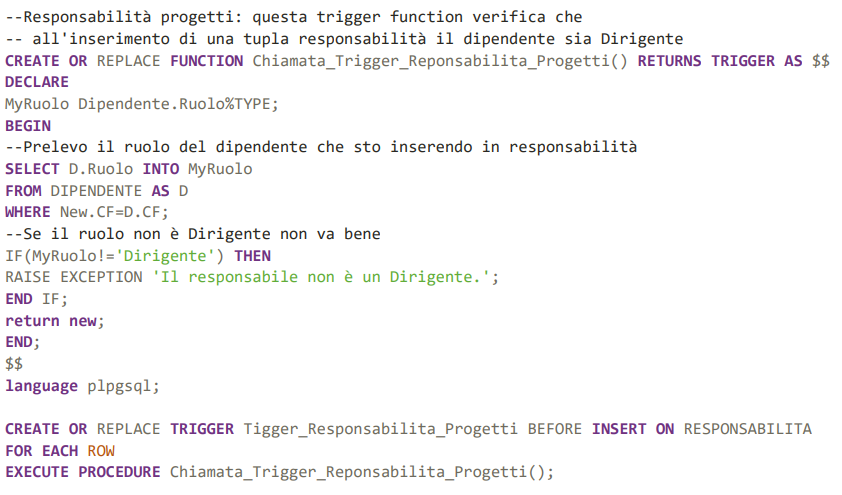
\includegraphics[width=1\textwidth]{Immagini/responsabilita.sql}
\newline\newline
Esempio di cosa accade se provo a responsabilizzare un dipendente non Dirigente:
\newline\newline
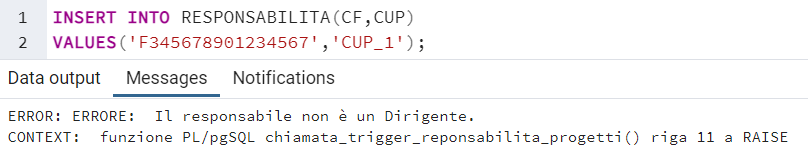
\includegraphics[width=1\textwidth]{Immagini/reses}
\subsection{Gestione Laboratori}
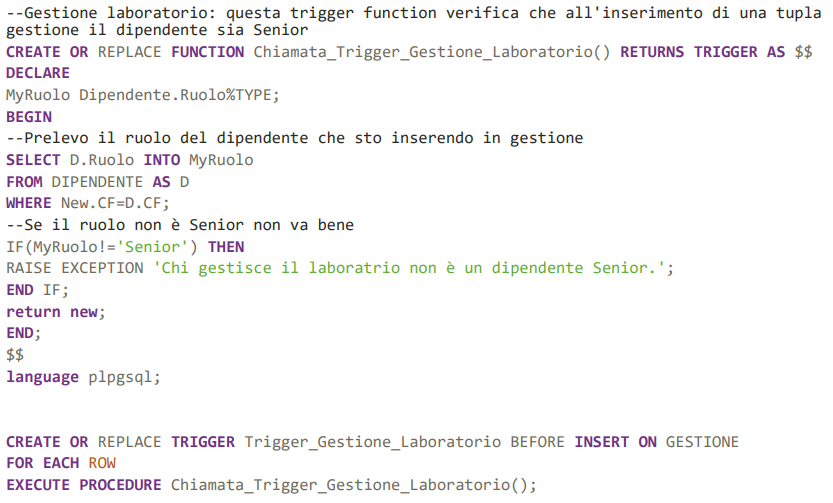
\includegraphics[width=1\textwidth]{Immagini/gestione.sql}
\newline\newline
Esempio di cosa accade se provo a far gestire un laboratorio da un dipendente non Senior:
\newline\newline
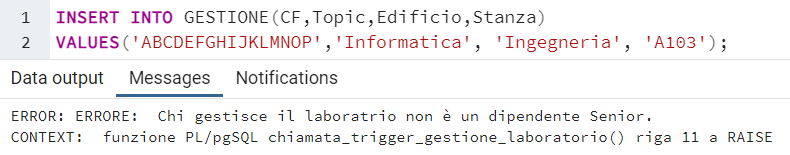
\includegraphics[width=1\textwidth]{Immagini/geses}
\subsection{Referenza Progetti}
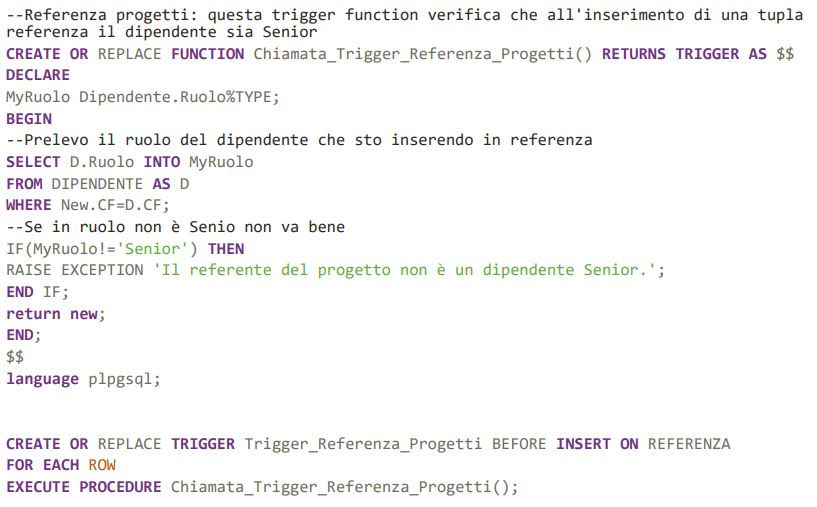
\includegraphics[width=1\textwidth]{Immagini/referenza.sql}
\newline\newline
Esempio di cosa accade se provo a far referenziare un progetto da un dipendente non Senior:
\newline\newline
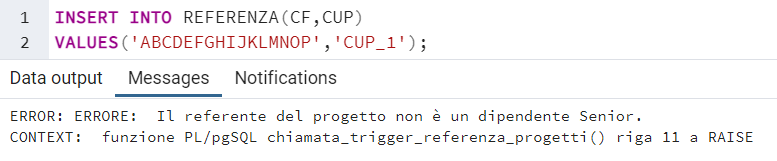
\includegraphics[width=1\textwidth]{Immagini/refes}



 
